\documentclass[11pt, oneside]{article}
\usepackage[letterpaper, margin=2cm]{geometry}
\usepackage{MATH667}
\usepackage{booktabs}
\newcommand{\doubletilde}[1]{\tilde{\tilde{#1}}}

\begin{document}
\noindent \textbf{\Large{Caleb Logemann \\
MATH667 Hyperbolic Partial Differential Equations \\
Final Project
}}

%\lstinputlisting[language=MATLAB]{H01_23.m}
\begin{enumerate}
  \item % #1
    Write out the Jacobian matrix and derive the eigenvalues and eigenvectors
    for the Euler equations.

    We have the following vector flux function written in terms of the conserved variables.
    \[
      \v{f}(\v{w}) =
      \begin{bmatrix}
        m \\
        \frac{m^2}{\rho} + P \\
        \frac{m}{\rho}\p{E + P}
      \end{bmatrix}
    \]
    where
    \[
      P = \p{\gamma - 1}\p{E - \frac{m^2}{2\rho}}
    \]
    or
    \[
      E = \frac{P}{\gamma - 1} + \frac{\rho u^2}{2}
    \]

    In order to compute the Jacobian of $\v{f}$ I will first compute the partial derivatives of $P$.
    \begin{align*}
      P_{\rho} &= \p{\gamma - 1} \frac{m^2}{2 \rho^2} \\
      P_m &= -\p{\gamma - 1}\frac{m}{\rho} \\
      P_E &= \gamma - 1
    \end{align*}
    Now the Jacobian of $\v{f}$ can expressed as
    \[
      \v{f}'(\v{w}) =
      \begin{bmatrix}
        0 & 1 & 0 \\
        -\frac{m^2}{\rho^2} + P_{\rho} & 2 \frac{m}{\rho} + P_m & P_E \\
        P_{\rho} \frac{m}{\rho} - (E + P)\frac{m}{\rho^2} & P_m \frac{m}{\rho} + (E + P) \frac{1}{\rho} & \frac{m}{p}\p{1 + P_E}
      \end{bmatrix}
    \]
    Simplifying this results in
    \[
      \v{f}'(\v{w}) =
      \begin{bmatrix}
        0 & 1 & 0 \\
        \p{\gamma - 3} \frac{m^2}{2 \rho^2} & \p{3 - \gamma}\frac{m}{\rho} & \gamma - 1 \\
        \p{\gamma - 1} \frac{m^3}{2 \rho^3} - m\frac{E + P}{\rho^2} & \frac{E + P}{\rho} - \p{\gamma - 1}\frac{m^2}{\rho^2}  & \gamma\frac{m}{p}
      \end{bmatrix}
    \]
    This can also be changed into primitive variables.
    \[
      \v{f}'(\v{w}) =
      \begin{bmatrix}
        0 & 1 & 0 \\
        \p{\gamma - 3} \frac{u^2}{2} & \p{3 - \gamma}u & \gamma - 1 \\
        \frac{1}{2}\p{\gamma - 2} u^3 - \frac{\gamma}{\gamma - 1}\frac{uP}{\rho} & \frac{\gamma}{\gamma - 1}\frac{P}{\rho} + \p{\frac{3}{2} - \gamma}u^2  & \gamma u
      \end{bmatrix}
    \]

    Now in order to find the eigenvalues and eigenvectors of this matrix we
    start by subtracting $\lambda I$ and solving
    $\det(\v{f}'(\v{w}) - \lambda I) = 0$.
    \begin{gather*}
      \det(\v{f}'(\v{w}) - \lambda I) =
      \begin{vmatrix}
        -\lambda & 1 & 0 \\
        \p{\gamma - 3} \frac{u^2}{2} & \p{3 - \gamma}u - \lambda & \gamma - 1 \\
        \frac{1}{2}\p{\gamma - 2} u^3 - \frac{\gamma}{\gamma - 1}\frac{uP}{\rho} & \frac{\gamma}{\gamma - 1}\frac{P}{\rho} + \p{\frac{3}{2} - \gamma}u^2  & \gamma u - \lambda \\
      \end{vmatrix} \\
      = -\lambda \p{\p{3 - \gamma}u - \lambda} \p{\gamma u - \lambda} + \p{\gamma - 1}\p{\frac{1}{2}\p{\gamma - 2} u^3 - \frac{\gamma}{\gamma - 1}\frac{uP}{\rho}} \\
      + \lambda \p{\gamma - 1} \p{\frac{\gamma}{\gamma - 1}\frac{P}{\rho} + \p{\frac{3}{2} - \gamma}u^2} - \p{\gamma - 3} \frac{u^2}{2}\p{\gamma u - \lambda}
      %= -\lambda \p{\p{3 - \gamma}u - \lambda} \p{\gamma u - \lambda} + \p{\gamma - 1}\p{\p{\gamma - 1} u^3 - uH} - (\gamma - 3)\frac{u^2}{2}\p{\gamma u - \lambda} + \lambda \p{\gamma - 1} \p{H - (\gamma - 1)u^2}
    \end{gather*}
    I will separate out each of these terms as
    \begin{align*}
      a_1 &= -\lambda \p{\p{3 - \gamma}u - \lambda} \p{\gamma u - \lambda} \\
      a_2 &= \p{\gamma - 1}\p{\frac{1}{2}\p{\gamma - 2} u^3 - \frac{\gamma}{\gamma - 1}\frac{uP}{\rho}} \\
      a_3 &= \lambda \p{\gamma - 1} \p{\frac{\gamma}{\gamma - 1}\frac{P}{\rho} + \p{\frac{3}{2} - \gamma}u^2} \\
      a_4 &= -\p{\gamma - 3} \frac{u^2}{2}\p{\gamma u - \lambda}
    \end{align*}
    so the determinant is $a_1 + a_2 + a_3 + a_4$.
    Now I will simplify each of these terms
    \begin{align*}
      a_1 &=  -\lambda \p{\p{3 - \gamma}u - \lambda} \p{\gamma u - \lambda} \\
      &= \p{\p{\gamma - 3}u\lambda + \lambda^2} \p{\gamma u - \lambda} \\
      &= \p{\gamma - 3}\gamma u^2 \lambda - \p{\gamma - 3} u\lambda^2 + \gamma u \lambda^2 - \lambda^3 \\
      &= \p{\gamma - 3}\gamma u^2 \lambda + 3u \lambda^2 - \lambda^3
    \end{align*}
    \begin{align*}
      a_2 &= \p{\gamma - 1}\p{\frac{1}{2}\p{\gamma - 2} u^3 - \frac{\gamma}{\gamma - 1}\frac{uP}{\rho}} \\
      &= \frac{1}{2}\p{\gamma - 1}\p{\gamma - 2} u^3 - \gamma\frac{uP}{\rho}
    \end{align*}
    \begin{align*}
      a_3 &= \lambda \p{\gamma - 1} \p{\frac{\gamma}{\gamma - 1}\frac{P}{\rho} + \p{\frac{3}{2} - \gamma}u^2} \\
      &= \lambda \p{\gamma\frac{P}{\rho} +\p{\gamma - 1}\p{\frac{3}{2} - \gamma}u^2}
    \end{align*}
    \begin{align*}
      a_4 &= -\p{\gamma - 3} \frac{u^2}{2}\p{\gamma u - \lambda} \\
      &= \lambda\p{\gamma - 3} \frac{u^2}{2} - \gamma \p{\gamma - 3}\frac{u^3}{2}
    \end{align*}
    Adding these all back together gives
    \begin{gather*}
      a_1 + a_2 + a_3 + a_4 = -\lambda^3 + 3u \lambda^2 \\
      + \p{\gamma\frac{P}{\rho} +\p{\gamma - 1}\p{\frac{3}{2} - \gamma}u^2 + \p{\gamma - 3}\p{\gamma + \frac{1}{2}} u^2}\lambda - \gamma \p{\gamma - 3}\frac{u^3}{2} + \frac{1}{2}\p{\gamma - 1}\p{\gamma - 2} u^3 - \gamma\frac{uP}{\rho}
    \end{gather*}
    Now I will simplify each of the coefficients of $\lambda$.
    \begin{align*}
      &\gamma\frac{P}{\rho} +\p{\gamma - 1}\p{\frac{3}{2} - \gamma}u^2 + \p{\gamma - 3}\p{\gamma + \frac{1}{2}}u^2 \\
      &= \gamma\frac{P}{\rho} + \p{\p{\gamma - 1}\p{\frac{3}{2} - \gamma} + \p{\gamma - 3}\p{\gamma + \frac{1}{2}}}u^2 \\
      &= \gamma\frac{P}{\rho} + \p{-\gamma^2 + \frac{5}{2}\gamma - \frac{3}{2} + \gamma^2 - \frac{5}{2}\gamma - \frac{3}{2}}u^2 \\
      &= \gamma\frac{P}{\rho} + -3u^2
    \end{align*}
    \begin{align*}
      &-\gamma \p{\gamma - 3}\frac{u^3}{2} + \frac{1}{2}\p{\gamma - 1}\p{\gamma - 2} u^3 - \gamma\frac{uP}{\rho} \\
      &= \p{-\gamma \p{\gamma - 3} + \p{\gamma - 1}\p{\gamma - 2}} \frac{u^3}{2} - \gamma\frac{uP}{\rho} \\
      &= \p{-\gamma^2 + 3\gamma + \gamma^2 - 3\gamma + 2} \frac{u^3}{2} - \gamma\frac{uP}{\rho} \\
      &=  u^3 - \gamma\frac{uP}{\rho}
    \end{align*}
    So now simplifying these terms by factoring into a difference cubed
    \begin{gather*}
      a_1 + a_2 + a_3 + a_4 = -\lambda^3 + 3u \lambda^2 + \p{\gamma\frac{P}{\rho} + -3u^2}\lambda + u^3 - \gamma\frac{uP}{\rho} \\
      = -\lambda^3 + 3u \lambda^2 - 3u^2\lambda + u^3 + \gamma\lambda\frac{P}{\rho} - \gamma\frac{uP}{\rho} \\
      = \p{u - \lambda}^3 - \p{u - \lambda} \frac{\gamma P}{\rho} \\
    \end{gather*}
    Thus we have shown that
    \[
      \det(\v{f}'(\v{w}) - \lambda I) = \p{u - \lambda}^3 - \p{u - \lambda} \frac{\gamma P}{\rho}
    \]
    Setting this equal to zero and solving for $\lambda$ gives.
    \begin{align*}
      \p{u - \lambda}^3 - \p{u - \lambda} \frac{\gamma P}{\rho} &= 0 \\
      \p{u - \lambda}\p{\p{u - \lambda}^2 - \frac{\gamma P}{\rho}} &= 0 \\
      \lambda &= u \\
      \p{u - \lambda}^2 - \frac{\gamma P}{\rho} &= 0 \\
      \p{u - \lambda}^2 &= \frac{\gamma P}{\rho} \\
      \p{u - \lambda} &= \pm\sqrt{\frac{\gamma P}{\rho}} \\
      \lambda &= u \pm\sqrt{\frac{\gamma P}{\rho}}
    \end{align*}
    So the three eigenvalues of this system are
    \[
      \lambda_1 = u, \quad \lambda_2 = u + \sqrt{\frac{\gamma P}{\rho}}, \quad \lambda_3 = u - \sqrt{\frac{\gamma P}{\rho}}
    \]

    Now I will just check that we have the correct eigenvectors.
    The eigenvectors are
    \[
      \v{w}_1 =
      \begin{bmatrix}
        1 \\
        u \\
        \frac{1}{2}u^2
      \end{bmatrix}, \quad
      \v{w}_2 =
      \begin{bmatrix}
        1 \\
        u + \sqrt{\frac{\gamma P}{\rho}} \\
        \frac{\gamma}{\gamma - 1}\frac{P}{\rho} + \frac{u^2}{2} + u\sqrt{\frac{\gamma P}{\rho}} \\
      \end{bmatrix}, \quad
      \v{w}_3 =
      \begin{bmatrix}
        1 \\
        u - \sqrt{\frac{\gamma P}{\rho}} \\
        \frac{\gamma}{\gamma - 1}\frac{P}{\rho} + \frac{u^2}{2} - u\sqrt{\frac{\gamma P}{\rho}} \\
      \end{bmatrix}
    \]
    To check
    \begin{align*}
      \v{f}' \v{w}_1 &= 
      \begin{bmatrix}
        0 & 1 & 0 \\
        \p{\gamma - 3} \frac{u^2}{2} & \p{3 - \gamma}u & \gamma - 1 \\
        \frac{1}{2}\p{\gamma - 2} u^3 - \frac{\gamma}{\gamma - 1}\frac{uP}{\rho} & \frac{\gamma}{\gamma - 1}\frac{P}{\rho} + \p{\frac{3}{2} - \gamma}u^2  & \gamma u
      \end{bmatrix}
      \begin{bmatrix}
        1 \\
        u \\
        \frac{1}{2}u^2
      \end{bmatrix} \\
      &=
      \begin{bmatrix}
        u \\
        (\gamma - 3)\frac{u^2}{2} - (\gamma - 3)u^2 + (\gamma - 1)\frac{u^2}{2} \\
        \frac{1}{2}\p{\gamma - 2} u^3 - \frac{\gamma}{\gamma - 1}\frac{uP}{\rho} + \frac{\gamma}{\gamma - 1}\frac{uP}{\rho} + \p{\frac{3}{2} - \gamma}u^3 + \gamma \frac{u^3}{2}
      \end{bmatrix} \\
      &= 
      \begin{bmatrix}
        u \\
        u^2 \\
        \frac{1}{2}u^3
      \end{bmatrix} \\
      &= u
      \begin{bmatrix}
        1 \\
        u \\
        \frac{1}{2}u^2
      \end{bmatrix}
    \end{align*}
    Let $c = \sqrt{\frac{\gamma P}{\rho}}$
    \begin{align*}
      \v{f}' \v{w}_2 &= 
      \begin{bmatrix}
        0 & 1 & 0 \\
        \p{\gamma - 3} \frac{u^2}{2} & \p{3 - \gamma}u & \gamma - 1 \\
        \frac{1}{2}\p{\gamma - 2} u^3 - \frac{\gamma}{\gamma - 1}\frac{uP}{\rho} & \frac{\gamma}{\gamma - 1}\frac{P}{\rho} + \p{\frac{3}{2} - \gamma}u^2  & \gamma u
      \end{bmatrix}
      \begin{bmatrix}
        1 \\
        u + c \\
        \frac{1}{\gamma - 1}c^2 + \frac{u^2}{2} + uc \\
      \end{bmatrix} \\
      &=
      \begin{bmatrix}
        u + c \\
        \p{\gamma - 3} \frac{u^2}{2} + \p{3 - \gamma}u\p{u + c} + \p{\gamma - 1}\p{\frac{1}{\gamma - 1}c^2 + \frac{u^2}{2} + uc} \\
        \frac{1}{2}\p{\gamma - 2} u^3 - \frac{\gamma}{\gamma - 1}\frac{uP}{\rho} + \p{\frac{\gamma}{\gamma - 1}\frac{P}{\rho} + \p{\frac{3}{2} - \gamma}u^2}\p{u + c} + \gamma u \p{\frac{1}{\gamma - 1}c^2 + \frac{u^2}{2} + uc}
      \end{bmatrix} \\
      &=
      \begin{bmatrix}
        u + c \\
        \p{\gamma - 3} \frac{u^2}{2} + \p{3 - \gamma}u^2 + \p{3 - \gamma}uc + c^2 + \p{\gamma - 1}\frac{u^2}{2} + \p{\gamma - 1}uc \\
        \frac{1}{2}\p{\gamma - 2} u^3 + uc^2 + \frac{1}{\gamma - 1}c^2\p{u+c} + \p{\frac{3}{2} - \gamma}u^3 + \p{\frac{3}{2} - \gamma}u^2c + \gamma\frac{u^3}{2} + \gamma u^2c
      \end{bmatrix} \\
      &=
      \begin{bmatrix}
        u + c \\
        u^2 + 2uc + c^2 \\
        \frac{1}{2} u^3 + \frac{1}{\gamma - 1}c^2\p{u+c} + \frac{3}{2}u^2c + uc^2
      \end{bmatrix} \\
      &=
      \begin{bmatrix}
        u + c \\
        \p{u + c}^2 \\
        \p{\frac{u^2}{2} + uc}\p{u + c} + \frac{1}{\gamma - 1}c^2\p{u + c}
      \end{bmatrix} \\
      &= (u + c)
      \begin{bmatrix}
        1 \\
        u + c \\
        \frac{1}{\gamma - 1}c^2 + \frac{u^2}{2} + uc
      \end{bmatrix} \\
    \end{align*}
    \begin{align*}
      \v{f}' \v{w}_3 &= 
      \begin{bmatrix}
        0 & 1 & 0 \\
        \p{\gamma - 3} \frac{u^2}{2} & \p{3 - \gamma}u & \gamma - 1 \\
        \frac{1}{2}\p{\gamma - 2} u^3 - \frac{\gamma}{\gamma - 1}\frac{uP}{\rho} & \frac{\gamma}{\gamma - 1}\frac{P}{\rho} + \p{\frac{3}{2} - \gamma}u^2  & \gamma u
      \end{bmatrix}
      \begin{bmatrix}
        1 \\
        u - c \\
        \frac{1}{\gamma - 1}c^2 + \frac{u^2}{2} - uc \\
      \end{bmatrix} \\
      &=
      \begin{bmatrix}
        u - c \\
        \p{\gamma - 3} \frac{u^2}{2} + \p{3 - \gamma}u\p{u - c} + \p{\gamma - 1}\p{\frac{1}{\gamma - 1}c^2 + \frac{u^2}{2} - uc} \\
        \frac{1}{2}\p{\gamma - 2} u^3 - \frac{\gamma}{\gamma - 1}\frac{uP}{\rho} + \p{\frac{\gamma}{\gamma - 1}\frac{P}{\rho} + \p{\frac{3}{2} - \gamma}u^2}\p{u - c} + \gamma u \p{\frac{1}{\gamma - 1}c^2 + \frac{u^2}{2} - uc}
      \end{bmatrix} \\
      &=
      \begin{bmatrix}
        u - c \\
        \p{\gamma - 3} \frac{u^2}{2} + \p{3 - \gamma}u^2 - \p{3 - \gamma}uc + c^2 + \p{\gamma - 1}\frac{u^2}{2} - \p{\gamma - 1}uc \\
        \frac{1}{2}\p{\gamma - 2} u^3 + uc^2 + \frac{1}{\gamma - 1}c^2\p{u-c} + \p{\frac{3}{2} - \gamma}u^3 - \p{\frac{3}{2} - \gamma}u^2c + \gamma\frac{u^3}{2} - \gamma u^2c
      \end{bmatrix} \\
      &=
      \begin{bmatrix}
        u - c \\
        u^2 - 2uc + c^2 \\
        \frac{1}{2} u^3 + \frac{1}{\gamma - 1}c^2\p{u-c} - \frac{3}{2}u^2c + uc^2
      \end{bmatrix} \\
      &=
      \begin{bmatrix}
        u - c \\
        \p{u - c}^2 \\
        \p{\frac{u^2}{2} - uc}\p{u - c} + \frac{1}{\gamma - 1}c^2\p{u - c}
      \end{bmatrix} \\
      &= (u - c)
      \begin{bmatrix}
        1 \\
        u - c \\
        \frac{1}{\gamma - 1}c^2 + \frac{u^2}{2} - uc
      \end{bmatrix} \\
    \end{align*}

  \item % #2
    \lstinputlisting[language=MATLAB]{finalProject.m}
    \lstinputlisting[language=MATLAB]{rungeKutta3.m}
    \lstinputlisting[language=MATLAB]{muscl3System.m}

    \begin{center}
      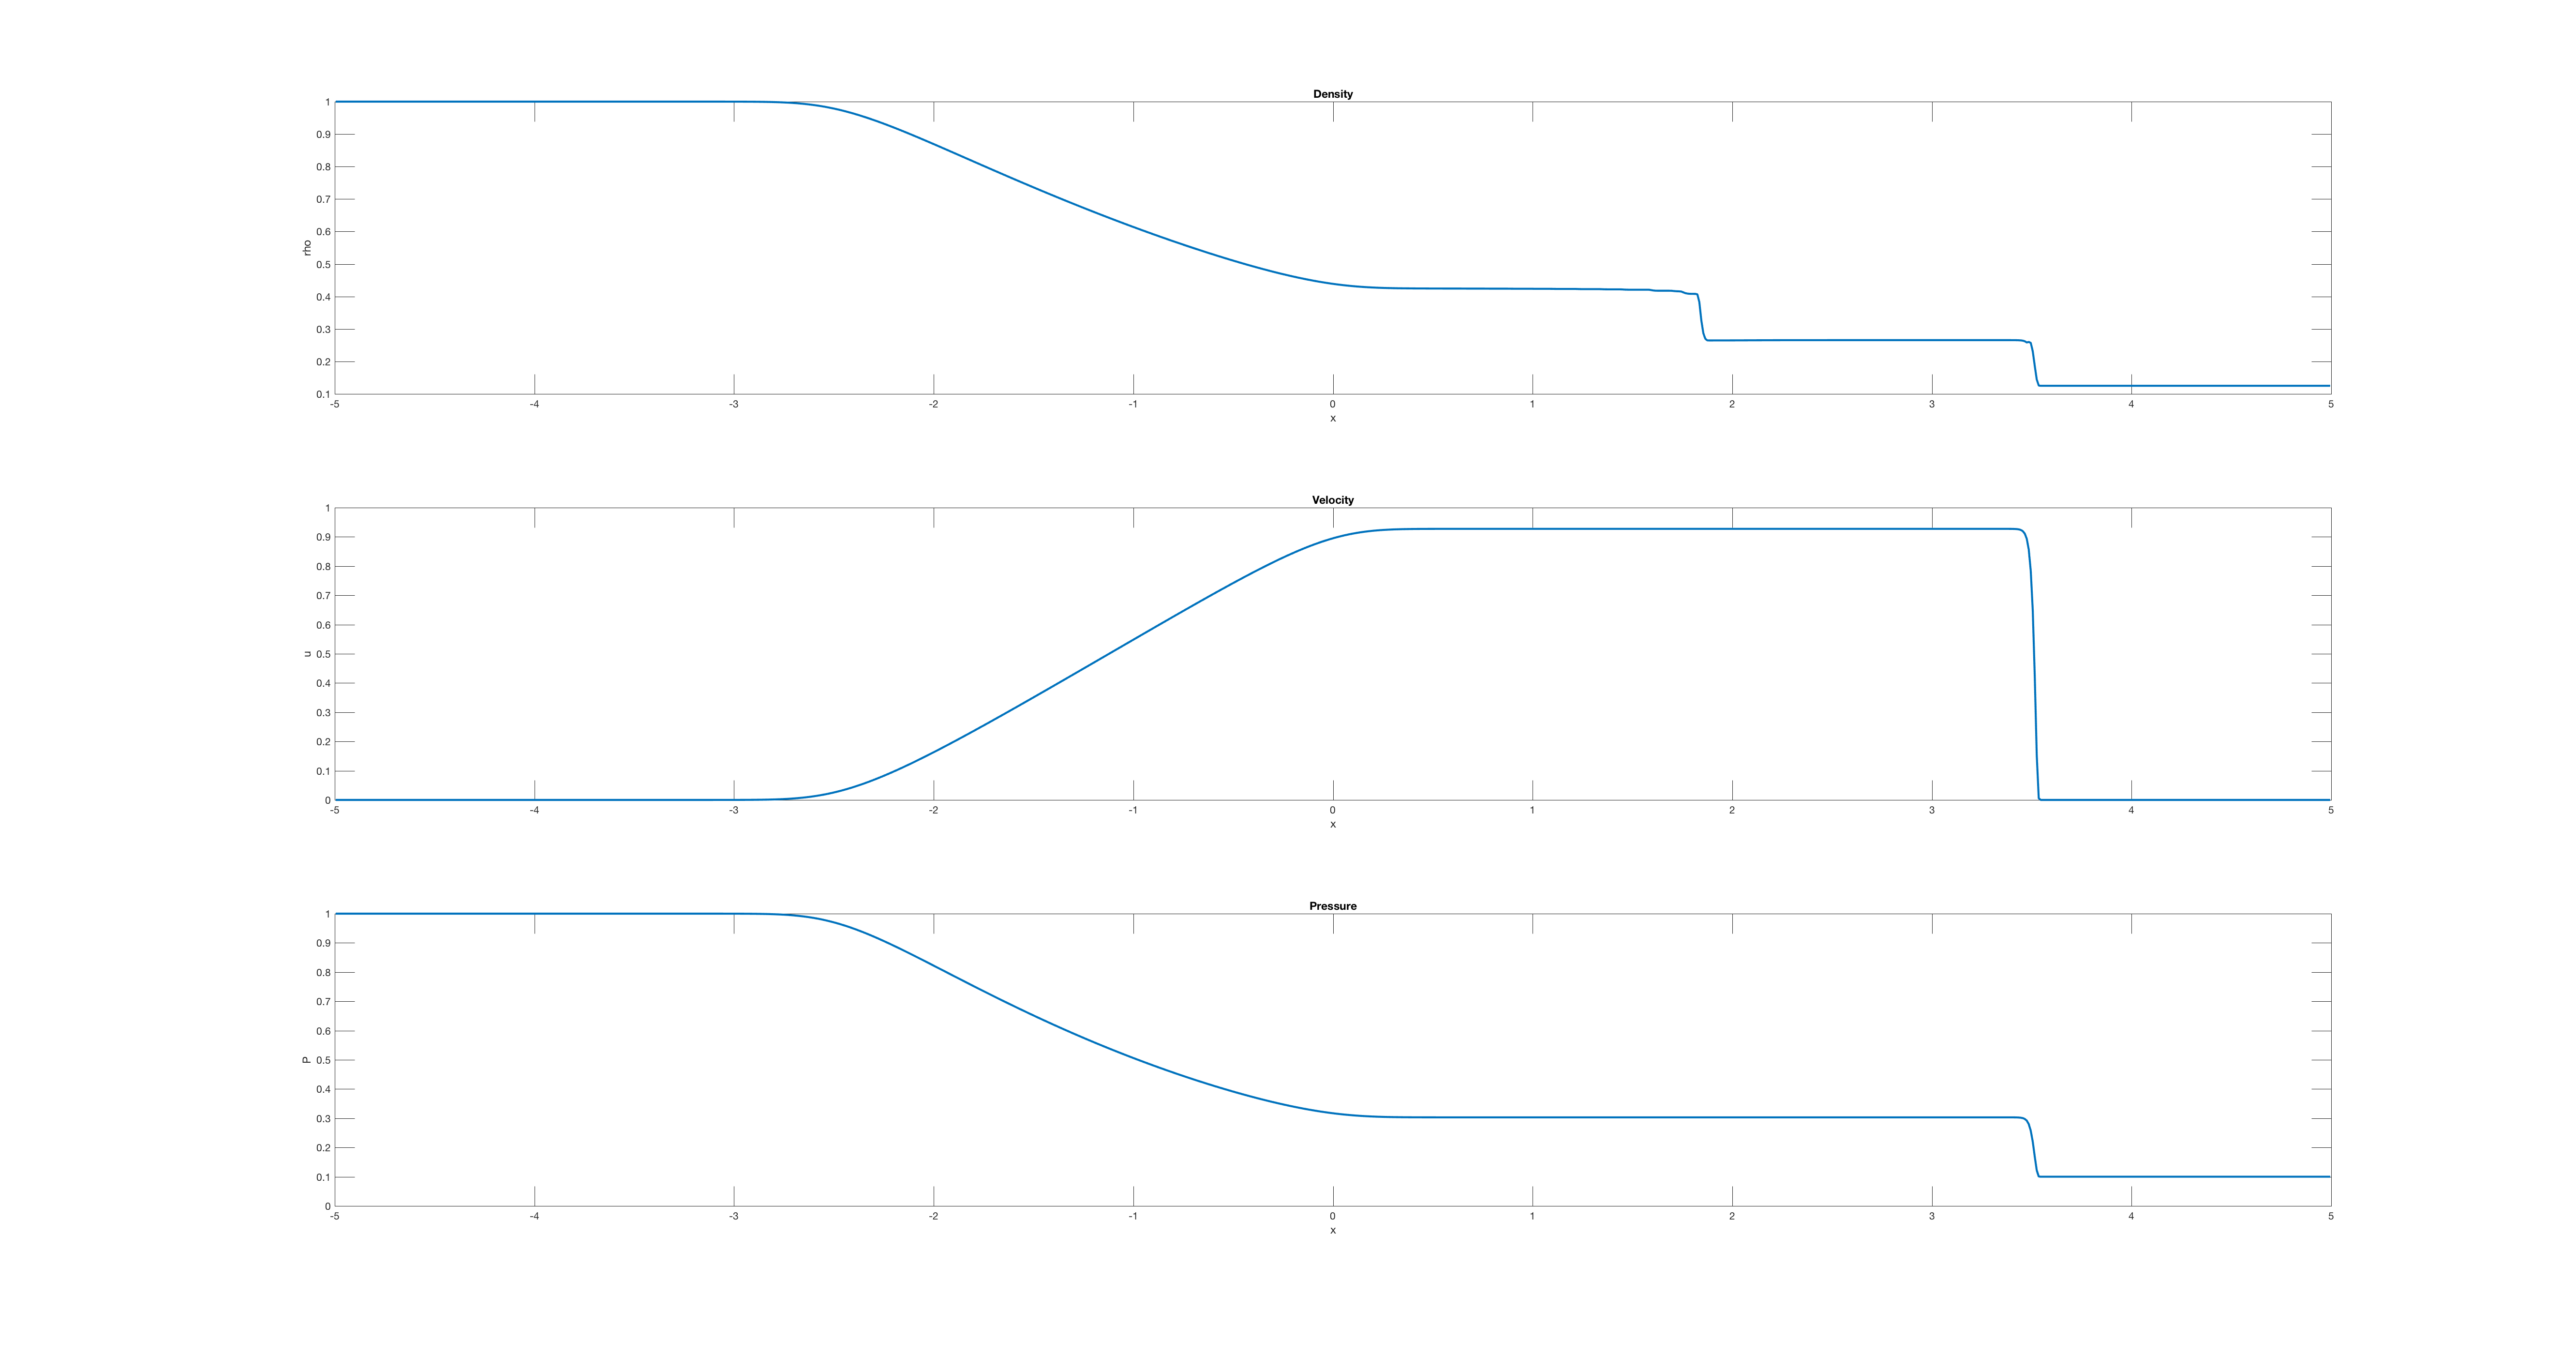
\includegraphics[scale=0.5]{Figures/finalProject.png}
    \end{center}
    
\end{enumerate}
\end{document}
